%%%%%%%%%%%%%%%%%%%%%%%%%%%%%%%%%%%%%%%%%
% Engineering Calculation Paper
% LaTeX Template
% Version 1.0 (20/1/13)
%
% This template has been downloaded from:
% http://www.LaTeXTemplates.com
%
% Original author:
% Dmitry Volynkin (dim_voly@yahoo.com.au)
%
% License:
% CC BY-NC-SA 3.0 (http://creativecommons.org/licenses/by-nc-sa/3.0/)
%
% Modificaciones por Roberto Cerdas
%
% Si desea utilizar notas al margen, favor leer los comentarios en las líneas 32 y % 52. Si desea colocar un logo, favor leer comentario en línea 54. El comando     % \marginnote{texto} introduce notas al margen.  
%
%%%%%%%%%%%%%%%%%%%%%%%%%%%%%%%%%%%%%%%%%

%----------------------------------------------------------------------------------------
%	PACKAGES AND OTHER DOCUMENT CONFIGURATIONS
%----------------------------------------------------------------------------------------

\documentclass[12pt,a4paper]{article} % Use A4 paper with a 12pt font size - different paper sizes will require manual recalculation of page margins and border positions

\usepackage[spanish]{babel} % Utilizar reglas de idioma español
\usepackage[utf8]{inputenc} % Use UTF-8 encoding
\usepackage{marginnote} % Required for margin notes
\usepackage{wallpaper} % Required to set each page to have a background
\usepackage{lastpage} % Required to print the total number of pages
%\usepackage[left=1.3cm,right=4.6cm,top=1.8cm,bottom=4.0cm,marginparwidth=3.4cm]{geometry} % Comentar la línea abajo y descomentar esta para usar notas al margen
\usepackage[left=1.3cm,right=1.3cm,top=1.8cm,bottom=4.0cm]{geometry} % Adjust page margins
\usepackage{amsmath} % Required for equation customization
\usepackage{amssymb} % Required to include mathematical symbols
\usepackage{xcolor} % Required to specify colors by name
\usepackage[square, comma, sort&compress]{natbib} % Use the natbib reference package - read up on this to edit the reference style; if you want text (e.g. Smith et al., 2012) for the in-text references (instead of numbers), remove 'numbers' 

\usepackage{fancyhdr} % Required to customize headers
\setlength{\headheight}{80pt} % Increase the size of the header to accommodate meta-information
\pagestyle{fancy}\fancyhf{} % Use the custom header specified below
\renewcommand{\headrulewidth}{0pt} % Remove the default horizontal rule under the header

\setlength{\parindent}{0cm} % Remove paragraph indentation
\newcommand{\tab}{\hspace*{2em}} % Defines a new command for some horizontal space

\newcommand\BackgroundStructure{ % Command to specify the background of each page
\setlength{\unitlength}{1mm} % Set the unit length to millimeters

\setlength\fboxsep{0mm} % Adjusts the distance between the frameboxes and the borderlines
\setlength\fboxrule{0.5mm} % Increase the thickness of the border line
\put(10, 10){\fcolorbox{black}{white!10}{\framebox(192,247){}}} % Main content box
%\put(165, 10){\fcolorbox{black}{blue!10}{\framebox(37,247){}}} % Margin box: Descomentar para utilizar notas al margen.
\put(10, 262){\fcolorbox{black}{white!10}{\framebox(192, 25){}}} % Header box
%\put(143, 263){\includegraphics[height=23mm,keepaspectratio]{logo}} % Logo box - maximum height/width: 25x42. Descomentar esta línea para usar logo.
}

%----------------------------------------------------------------------------------------
%	HEADER INFORMATION
%----------------------------------------------------------------------------------------

\fancyhead[L]{\begin{tabular}{l r | l r} % The header is a table with 4 columns
\textbf{Proyecto} & Localizador Acústico & \textbf{Página} & \thepage/\pageref{LastPage} \\ % Project name and page count
\textbf{Trabajo} & Divisor & \textbf{Actualizado en:} & 08/12/2013 \\ % Job number and last updated date
\textbf{Versión} & 1 & \textbf{Revisado en:} & -/-/201- \\ % Version and reviewed date
\textbf{Diseñador} & Roberto Cerdas Robles & \textbf{Revisado por:} & Alfonso Chacón Rodríguez \\ % Designer and reviewer
\end{tabular}}

%----------------------------------------------------------------------------------------

\begin{document}

\AddToShipoutPicture{\BackgroundStructure} % Set the background of each page to that specified above in the header information section

%----------------------------------------------------------------------------------------
%	DOCUMENT CONTENT
%----------------------------------------------------------------------------------------

\section{Resumen} 

\section{Introducción} 

%\marginnote{All units are \\ \textbf{[kN, mm]}}

Este documento describe la implementación de un divisor para calcular la función:

\begin{equation}\label{eqn:divisor}
y=\frac{1}{x}
\end{equation}

Este bloque debe interfazarse con otras unidades de cálculo para la determinación de el ángulo de arribo de una señal acústica. En particular, hay una sección que debe calcular la correlación entre dos señales que arriban a un arreglo de micrófonos. Esta sección necesita realizar varias cálculos aritméticos, que dependen de la operación indicada por la eq. \ref{eqn:divisor}. 


\section{Especificaciones}

El bloque a diseñar en este proyecto debe entregar los resultados de la operación descrita por la eq. \ref{eqn:divisor}. El sistema debe tener una resolución de al menos 16 bits. Para su interconexión con las demás etapas, se especifican las siguientes entradas y salidas:\newline

\begin{tabular}{c||c||c}
Señal & Designación & Función\\
\hline
\hline
clk & input & Señal de reloj. \\
reset & input & Señal de reset, activa en bajo. \\
data\_in & input & Señal de control, sync\_in, activar para iniciar operación. \\
D & input & Datos de entrada. \\
\hline
Out & output & Datos de salida. \\
error & output & Señal de control, informa si hubo un error (División por cero u overflow). \\
data\_valid & output & Señal de control, sync\_out, indica que puede leerse la salida. \\
\end{tabular}

\section{Descripción de unidades a diseñar}

Se propone utilizar el algoritmo SRT  (Sweeney, Robertson, y Tocher) de radix-4 con máxima redundancia, alterado para calcular 8 bits por iteración (a diferencia del caso estándar, 2 bits por iteración). La ecuación para el cálculo del resultado parcial es:

\begin{equation}\label{eqn:SRT}
R_{i+1}=4R_i+q_i*D
\end{equation}

Donde $q_i$ es el bit de cociente generado por cada etapa; al utilizar máxima redundancia, existen siete cocientes posibles, conocidos como \emph{bits de cociente}, representados en notación redundante:

\begin{equation}\label{eqn:quotientbits}
q_i \in [-3,-2,-1,0,1,2,3]
\end{equation}

Es importante definir que el término \emph{bit de cociente} se usa de igual manera que en la literatura, es decir, expresa un bit en notación redundante, no en binario. Cada bit de cociente requiere de tres bits para ser expresado en binario \citep{Wey1999}. El bloque opera para valores de entrada $x$ dentro del rango:

\begin{equation}\label{eqn:range}
x \in ]0,2[
\end{equation}

El bloque está diseñado para aceptar 16 bits de entrada, en formato de punto fijo, con 1 bit de parte entera y 15 bits de parte fraccional. Por tanto, el rango de salida es de:

\begin{equation}\label{eqn:outrange}
y \in ]0.5;2^{15}[
\end{equation}

El rango se definió para utilizar el bloque con la mantisa de un número en formato de punto flotante.

\section{Especificaciones}

El bloque cuenta con las siguientes entradas y salidas:\newline

\begin{tabular}{c||c||c}
Señal & Designación & Función\\
\hline
\hline
clk & input & Señal de reloj. \\
reset & input & Señal de reset, activa en bajo. \\
data\_in & input & Señal de control, sync\_in, activar para iniciar operación. \\
D & input & Datos de entrada. \\
\hline
Out & output & Datos de salida. \\
error & output & Señal de control, informa si hubo un error (División por cero u overflow). \\
data\_valid & output & Señal de control, sync\_out, indica que puede leerse la salida. \\
\end{tabular}

\section{Descripción funcional de unidades}

La figura \ref{fig:Bloques} muestra un diagrama de bloques del sistema creado. Se describe el diseño a continuación:

\begin{figure}[htbp]
  \centering
    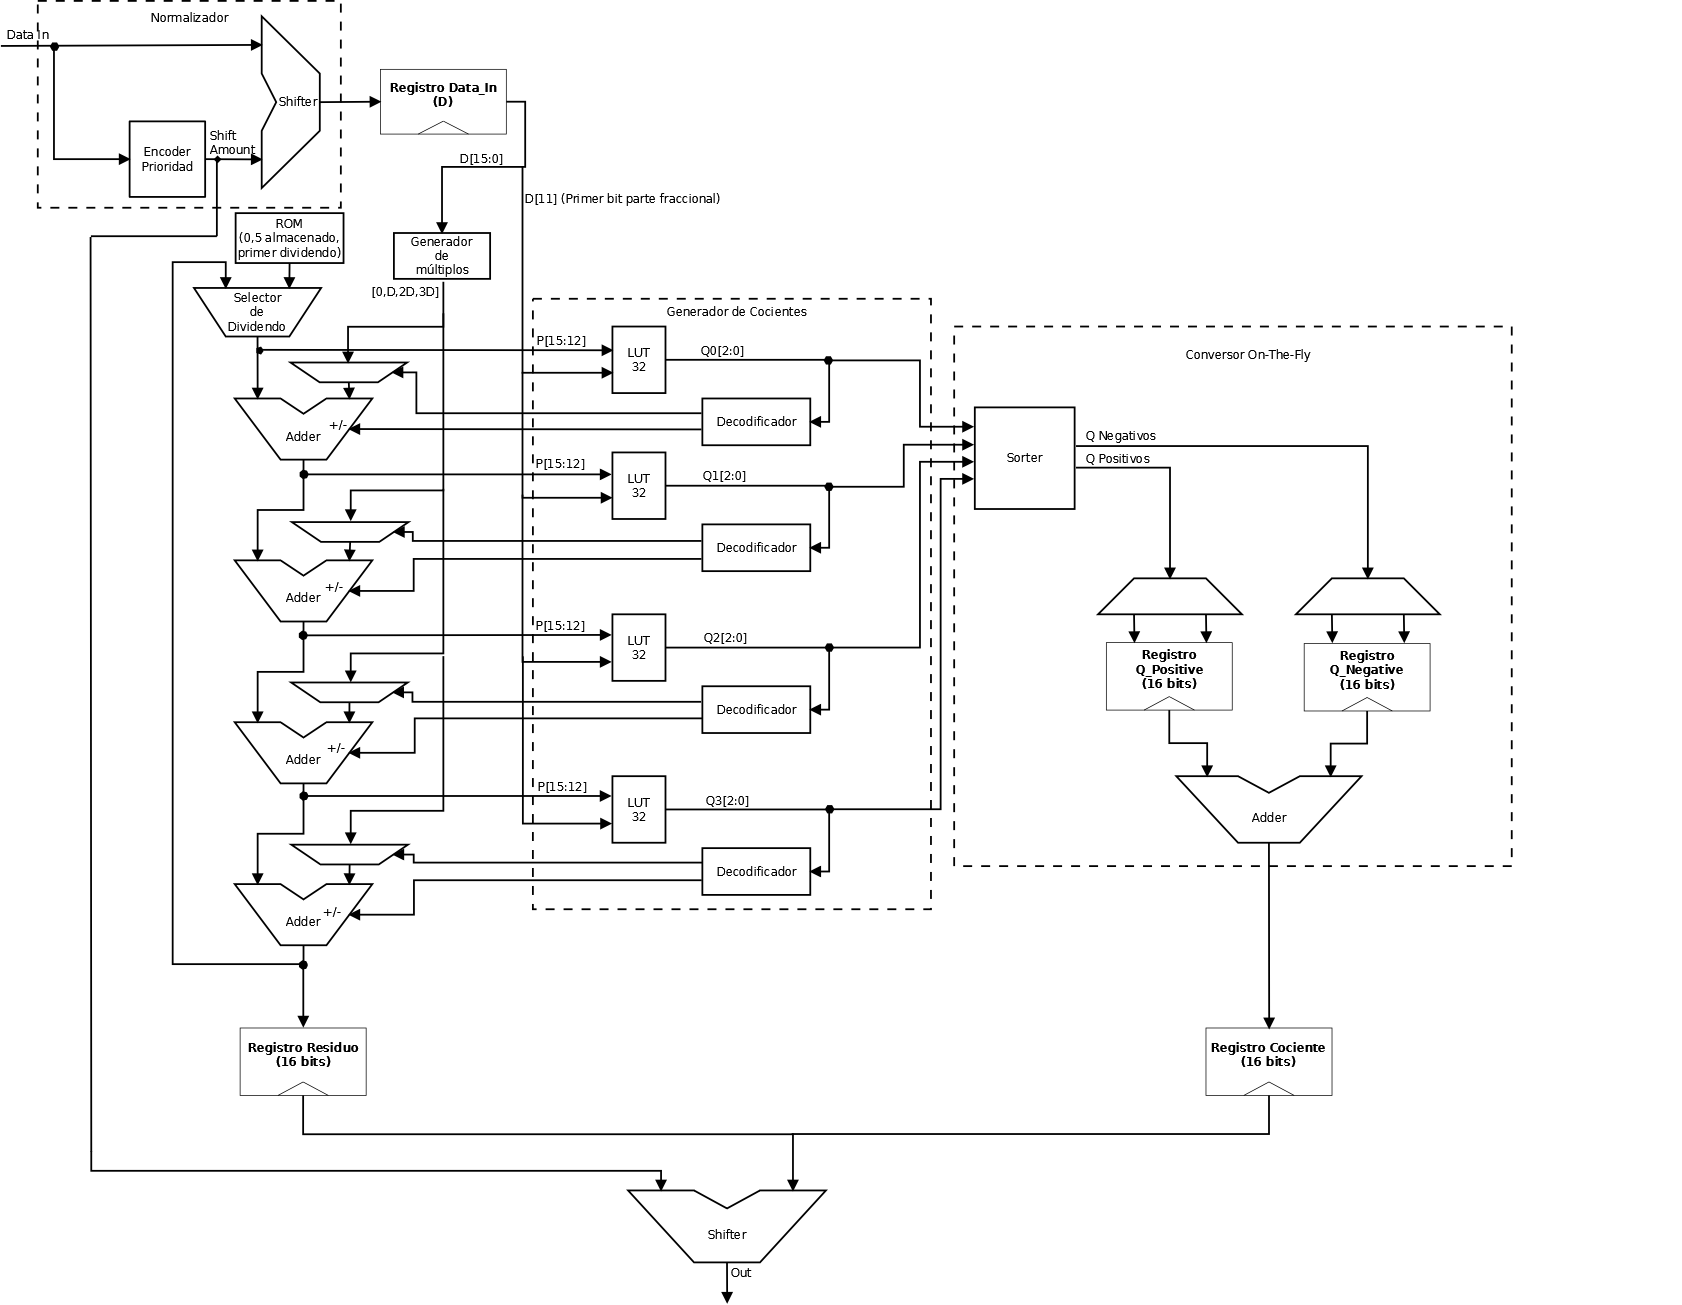
\includegraphics[scale=0.385, angle=270]{./Divisor.png}
    \rule{35em}{0.5pt}
  \caption[Bloques]{Diagrama de bloques del divisor realizado.}
  \label{fig:Bloques}
\end{figure}

\subsection{Normalizador}

El normalizador recibe un dato de entrada y lo normaliza al rango utilizado por el divisor, para cumplir con las restricciones del algoritmo SRT:

\begin{itemize}
\item[•]El divisor debe ser mayor al dividendo en cualquier iteración dada.
\item[•]El dividendo y los residuos parciales se multiplican por cuatro entre etapas.
\end{itemize}

La cantidad de corrimientos realizada en esta etapa se almacena para denormalizar el resultado a la salida del bloque.

\subsection{Generador de múltiplos}

Como se describió en la ecuación \ref{eqn:SRT}, el algoritmo requiere calcular el producto:

\begin{equation*}\label{eqn:productoD}
q_i*D
\end{equation*}

Para evitar repetir el cálculo cada vez que cambia el bit de cociente seleccionado, se calculan únicamente los valores $0,D,2D$ y $3D$:

\begin{itemize}
\item[•]0: Valor constante.
\item[•]D: El valor registrado a la entrada.
\item[•]2D: El valor registrado a la entrada, desplazado una posición.
\item[•]3D: La suma de los dos valores calculados anteriormente.
\end{itemize}

De esta forma, se puede acceder a los siete bits de cociente posibles sin implementar un multiplicador, utilizando únicamente corrimientos. Los valores de divisores posibles se envían a las entradas de las unidades de suma, donde el término apropiado es seleccionado por un multiplexor, y su signo se implementa realizando un complemento a 2 dentro del sumador al recibir la señal apropiada.

\subsection{Generador de cocientes}

El generador de cocientes toma el resultado parcial y el rango del divisor para seleccionar el bit de cociente apropiado para cada etapa. En la literatura, se determinó anteriormente que para un divisor de radix 4 de máxima redundancia, se requiere analizar únicamente los cuatro bits más significativos del resultado parcial anterior y un bit del divisor, para determinar si el divisor normalizado es mayor a $1,5$ \citep{Wey1999}. El bloque se implementa mediante el uso de LUT de 32 posiciones por etapa. Los rangos determinados en los que cada bit de cociente es válido se muestran a continuación:\newline

\begin{tabular}{c||c||c}
Resultado parcial & Valor de divisor & Bit de cociente\\
anterior $(R_i)$ & normalizado $(D)$ & $(q_i)$\\
\hline
\hline
$R_i\leq -3$ & $<1.5$ & $-3$. \\
$-3<R_i\leq -2$ & $<1.5$ & $-2$. \\
$-2<R_i\leq -1$ & $<1.5$ & $-1$. \\
$-1<R_i < 1$ & $<1.5$ & $0$. \\
$1\leq R_i < 2$ & $<1.5$ & $1$. \\
$2\leq R_i < 3$ & $<1.5$ & $2$. \\
$R_i \geq 3$ & $<1.5$ & $3$. \\
\hline
$R_i\leq -4$ & $\geq 1.5$ & $-3$. \\
$-4<R_i\leq -2$ & $\geq 1.5$ & $-2$. \\
$-2<R_i\leq -1$ & $\geq 1.5$ & $-1$. \\
$-1<R_i < 1$ & $\geq 1.5$ & $0$. \\
$1\leq R_i < 2$ & $\geq 1.5$ & $1$. \\
$2\leq R_i < 4$ & $\geq 1.5$ & $2$. \\
$R_i \geq 4$ & $\geq 1.5$ & $3$. \\
\end{tabular}

\subsection{Conversor On-The-Fly}

Para evitar utilizar una propagación con carry en cada etapa al sumar el bit de cociente seleccionado al resultado, se implementó un conversor que toma los bits en su representación redundante y calcula el cociente a partir de los mismos. Este conversor separa primero los bits en positivos y negativos, para así utilizar únicamente dos bits para representar cada valor. No se alteran los valores de los mismos; es decir, los bits negativos permanecen en complemento a 2, sin su bit de signo. \\

A continuación, se asigna un peso a cada par de bits, el cual corresponde a la etapa en la que fue generado el bit. Las etapas posteriores generan bits más significativos, y por tanto, se le asigna a los mismos mayor peso. Dos registros de 16 bits almacenan los resultados parciales; se genera un byte por iteración. Al finalizar ambas iteraciones, se suman los contenidos de ambos registros y se obtiene el cociente de la división.

\subsubsection{Sorter}

El separador de signos se implementa mediante una función lógica, realizando el \emph{AND} del bit de signo con cada uno de los bits restantes pertenecientes al bit de cociente para la salida negativa, repitiendo la operación con el bit de signo negado para la salida positiva.

\subsubsection{Asignación de pesos}

Los pesos se asignan concatenando los bits de cociente, de dos bits cada uno a la salida del sorter, en una palabra de 8 bits, colocando los de más peso en la posición más significativa. 

\subsection{Salida}

A la salida del bloque, se obtiene un valor positivo en el rango dado por \ref{eqn:outrange}. La palabra de salida es de 32 bits, en punto fijo, con 31 bits de parte entera y 33 bits de parte fraccional, denormalizada a su valor original.

\section{Datos y resultados}

\subsection{Temporizado}

La figura \ref{fig:Sim} muestra una simulación funcional del bloque, utilizando ModelSim:

\begin{figure}[htbp]
  \centering
    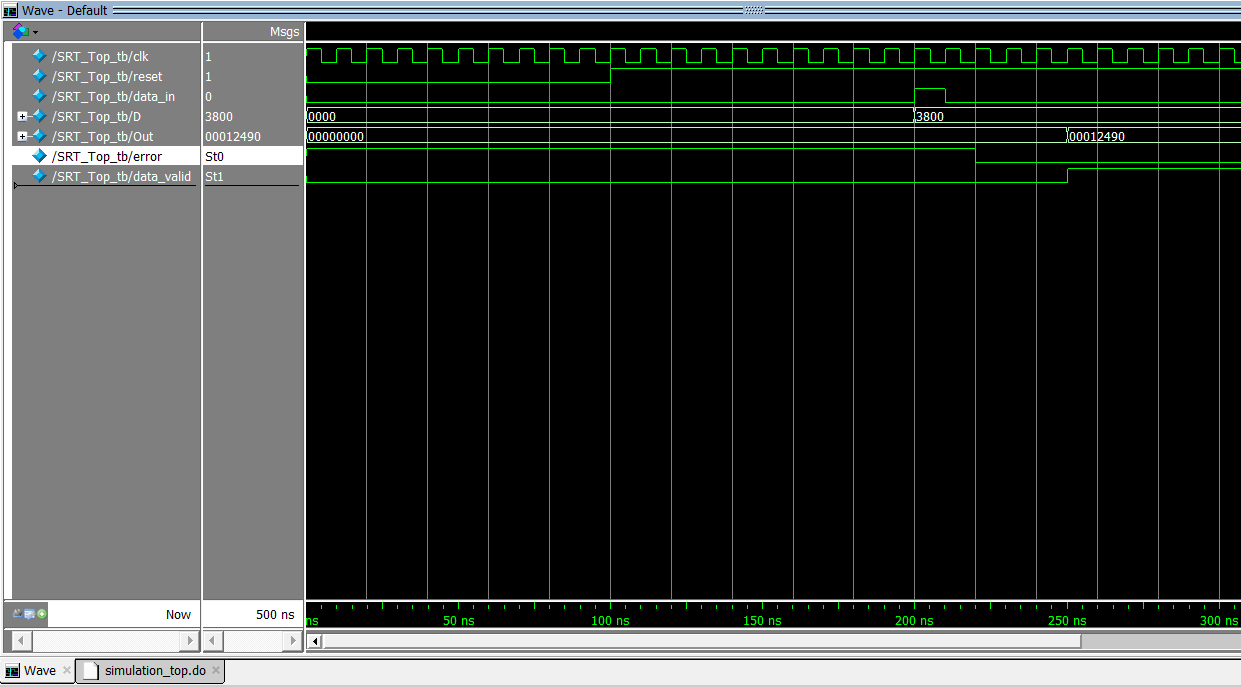
\includegraphics[scale=0.7]{./Simulation.png}
    \rule{35em}{0.5pt}
  \caption[Sim]{Simulación funcional del divisor SRT de radix 4 con máxima redundancia implementado.}
  \label{fig:Sim}
\end{figure}

\section{Análisis de datos y resultados}

Se puede observar en la  \ref{fig:Sim}  que el sistema es funcional a nivel de RTL.

Aquí se debe realizar un análisis de los sistemas desarrollados en términos de su cumplimiento de especificaciones (potencia, velocidad, área). Es decir, qué porcentaje de funcionalidad alcanzó el sistema, donde hay errores por corregir (y proponer su posible corrección) y que etapas podrían optimizarse. 

\section{Hoja de datos de unidades desarrolladas}

Describa brevemente (mejor en una tabla) las especificaciones finales del circuito (en términos de velocidad interna, velocidad de las interfaces, anchos y tipos de palabra usados, etc.). Además, en una tabla, describa la funcionalidad de cada pin del circuito y su protocolo de interconexión (por ejemplo: Pin RST, señal de reinicio del sistema, activa en bajo. La señal debe estar en bajo por al menos tres ciclos de reloj para alcanzar una reinicialización completa del sistema).

\section{Conclusiones y recomendaciones}

Aquí van las conclusiones y recomendaciones del Lab.

%----------------------------------------------------------------------------------------
\begin{thebibliography}{3}

\bibliographystyle{unsrtnat} % Use the "unsrtnat" BibTeX style for formatting the Bibliography

\bibitem[Wey(1999)]{Wey1999}
C.-L.Wey and C.-P.Wang
\newblock {Design of a fast radix-4 SRT divider and its VLSI implementation}.
\newblock \emph{IEEE Proc.-Comput. Digit. Tech., IEEE}, July 1999.
\newblock DOI: 10.1049/ip-cdt:19990524.

\end{thebibliography}

\end{document}